\documentclass{roles}

\title{Using Image Analysis and Machine Learning\\for Biodiversity Monitoring}
\author{Joe Collins - j.collins@zengenti.com}
\date{14 December 2023}

\begin{document}

\maketitle

\section*{Background}

In 2019, the Spains Hall Estate, Essex,
initiated a nature recovery and natural flood management program by introducing beavers,
into a fenced enclosure
\footnote{Spains Hall natural flood management \href{https://www.spainshallestate.co.uk/nfm\_beavers}{https://www.spainshallestate.co.uk/nfm\_beavers}}.
Comprehensive monitoring of the hydrology, canopy cover, and botanical species composition
has been conducted each year (2019-2023)
to assess the impact of beavers within the enclosure.
In the summer of 2023, more beavers were introduced into two further enclosures.
Survey data from the first enclosure will be used to generate a statistical model
to predict the timeline for impacts on woodland cover, changes in water levels
and botanical changes in the new enclosures.
This model will be used potential future
Biodiversity Net Gain calculations and improvements in Ecosystem Services. 



As changes take place in the two additional enclosure
the predictions provided by the statistical model will need to be checked against actual changes.
A full botanical survey is time consuming and requires extensive botanical identification skills.
Such a detailed approach is also unnecessary,
it would be reasonable to assume that the appearance





less demanding approach is required.
It is hoped that appropriate image analysis will serve this purpose.
As part of the surveys of the first enclosure,
two standardized geolocated full colour images were taken at each survey point
capturing canopy cover (light) and ground cover of vegetation,
bare ground and/or open water.

\begin{figure}[H]
  \centering
  \begin{tabular}{cc}
    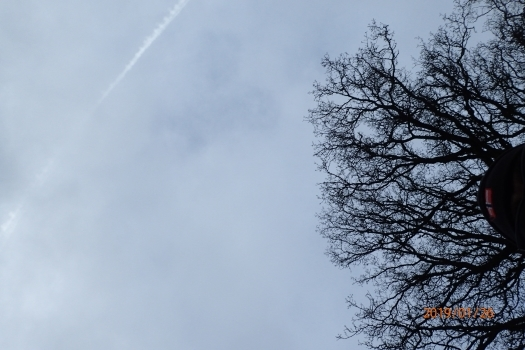
\includegraphics[width=0.45\linewidth]{../images/survey-up.jpg} &
    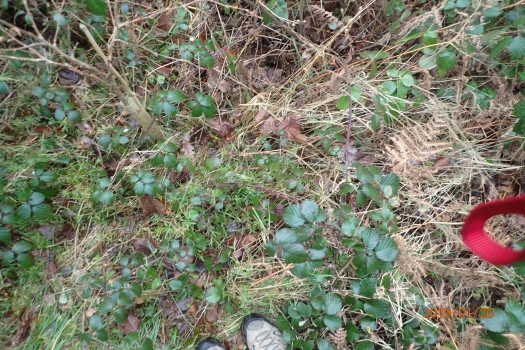
\includegraphics[width=0.45\linewidth]{../images/survey-down.jpg} \\
    Canopy Cover & Ground Cover\\
  \end{tabular}
\end{figure}

The collection of images will be used to create a second model which predicts changes
solely from features in the images.
The 





The model will be truthed against the real survey data and aims to predict changes in biodiversity,
which will enable the utilization of beavers as bioengineers within Biodiversity Net Gain calculations and Ecosystem Services. 

\section*{Objective}

Utilize machine learning techniques to predict Ellenberg indicator values (EIVs)
from geolocated images.
The focus is on automatically extracting features,
such as shape descriptors and leaf area index,
to generate a model predicting EIVs for images from the two additional enclosures.

\section*{Team}

Whilst the Spains Hall estate is a commercial enterprise,
this is a volunteer lead study
run by a collaborative team consisting of:

\begin{description}
    \item[Sarah Brockless] Ecologist \href{https://www.linkedin.com/in/sarah-brockless-833291a7/}{https://www.linkedin.com/in/sarah-brockless-833291a7/}.
    \item[Joe Collins] Software Engineer \href{https://www.linkedin.com/in/joejcollins/}{https://www.linkedin.com/in/joejcollins/}.
    \item[Mags Cousins] Botanist \href{https://www.researchgate.net/profile/Mags-Cousins}{https://www.researchgate.net/profile/Mags-Cousins}
    \item[David Gasca] Hydrologist \href{https://www.linkedin.com/in/david-gasca-7830537/}{https://www.linkedin.com/in/david-gasca-7830537/}.
\end{description}

The team would welcome input from a data scientist.

\section*{Opportunity Details}

\begin{description}
    \item[Data Availability] This is an open source project and
        the data thus far is available on \href{https://github.com/joejcollins/atlanta-shore}{https://github.com/joejcollins/atlanta-shore}.
    \item[Tools] The project uses both R and Python for data preparation and statistical analysis.
        Some familiarity with Git is needed but training can be given.
    \item[Survey Assistance] There will be an opportunity to assist with the botanical survey
        and data collection on site at the Spains Hall Estate, 20-24 June 2024.
    \item[Contact] For further information contact Joe Collins at \href{mailto:j.collins@zengenti.com}{j.collins@zengenti.com}.
\end{description}

\end{document}
